% ----------------------------
% Ian MacKay and Oamar Kanji
% Clustering and Linear Models
% MATH 4990 Final Project
% ----------------------------
\documentclass[12pt]{article}
\usepackage{color,graphicx}
\usepackage{hyperref}
\usepackage{minted}
\usepackage{tabular}

\setlength{\oddsidemargin}{0in}
\setlength{\evensidemargin}{0in}
\setlength{\topmargin}{0in}
\setlength{\textwidth}{6.5in}
\setlength{\textheight}{9in}

% -----
% Start
% -----
\begin{document}
\title{\vspace{-1.5in} Time Series Models and Object Clustering}
\author{Oamar Kanji \& Ian MacKay}
\maketitle

\tableofcontents

\section {Introduction}
  \par The first section of this report will seek to show that the initialization step in \textit{k}-means clustering is non-trivial, as the initial positions chosen for cluster means can significantly affect the final classification of the data set. The second section of this report will explore the use of ARIMA models in the analysis of Bitcoin prices, and some other methods of time series analysis.

\pagebreak

% ----------
% Clustering
% ----------
\section {Clustering}
  \par Clustering is the act of separating data into discrete groups to help analysis and prediction. It is also used for several compression and quantization algorithms, which are very important for image files. The resultant groups in k means clustering is highly dependent upon the method of centroid initialization.

\subsection {k-means}
  \par In its simplest form, \textit{k}-means assigns initial cluster means randomly. k data points are sampled from the data set and assigned as the initial positions for the centroids, thus sampling from a uniform distribution where every datapoint has an equal chance of being chosen.

\subsection {k++means}
  \par Proposed in 2007 by David Arthur and Sergei Vassilvitskii\cite{km_1}, \textit{k++}-means clustering seeks to reduce the inconsistency and increase the accuracy of the \textit{k}-means algorithm with a more sophisticated initialization. The general idea of this algorithm is to initialize centroids far away from each other such that multiple centroids are unlikely to find themselves within a single cluster that would lead to a local optimum.

  \par Unlike regular \textit{k}-means where initial centroids are sampled from a uniform distribution, \textit{k++} initializes centroids by sampling from a weighted distribution where the probability of a data point being chosen is proportionate to its distance from all other centroids.

  \par The initialization step is performed as follows:
  \begin{center}
    Let \textit{x} be an element of \textbf{x}, a subset of the data set whose elements are closest to the last chosen centroid. Then let \textbf{D}(\textit{x}) denote the shortest distance from a data point to the last center we have already chosen.
  \end{center}
  \begin{enumerate}
  \item Choose the first center uniformly at random from among the data points.
  \item For each data point \textit{x}, compute \textbf{D}(\textit{x}) the distance between \textit{x} and the nearest center that has already been chosen.
  \item Choose one new data point at random as a new centre, using a weighted probability distribution where a point \textit{x} is chosen with probability of choosing \textit{x} proportional to $\frac{\mathbf{D}(\mathit{x})^2}{\sum \limits_{\mathit{x} \in \mathbf{X}} \mathbf{D}(\mathit{x})^2}$, i.e the distance from x to the last centroid over the sum of the distances of all the points closeset to the last centroid.
  \item Repeat steps 2 and 3 until \textit{k} centers have been chosen.
  \item Now that the initial centers have been chosen, proceed using standard \textit{k}-means clustering.
  \end{enumerate}

\subsection {Initialization}
  The sum of squared error (henceforth referred to as SSE) can be calculated as follows:\\
  $SSE=\sum \limits_{i=1}^k \sum \limits_{p \in C_i} (p-m_i)^2$
  \begin{itemize}
    \item (k) number of clusters
    \item (C) set of objects in cluster
    \item (m) center point (mean) of cluster
  \end{itemize}

  \par Let us assume that for a particular value of k there exists \textbf{\textit{k} final centroids} that will result in the data set being clustered in a way that will minimize the SSE. Let us refer to these \textit{k} clusters as the \textbf{\textit{k} best fitting clusters} as they give a SSE that is small for that particular value of k. An example of this best case classification is shown in Figure 2.4.1.

  \par Sometimes, one or more centroids find what what is called a \textit{local optimum}. This is usually brought about by centroids that are initialized close to each other, which influences the final classification of data points to an extent that the SSE is large, as seen in Figure 2.4.2. In these examples, two initialized centroids do not find their way to the best fitting clusters. Instead, the two centroids remain close to each other, partitioning what should be a single cluster into two. As these leaves one ideal cluster out, it forces one of the remaining centroids to group two clusters together, resulting in an enlarged SSE.

  \par To observe the spread of results returned by \textit{k}-means clustering, the algorithm was repeated 100 times on the data set and the resultant centroids were plotted on top. This is shown in Figure 2.4.3. It can be observed that the areas of highest densities of plotted centroids lie over the four best clusters in the dataset. This may indicate that \textit{k}-means achieves finding the four best clusters on most runs, but there is a noticeable amount of dispersion of centroids which shows that the algorithm is inconsistent. This is a direct consequence of the method of initialization used in plain \textit{k}-means clustering.

  \par The histogram of SSE is shown in Figure 2.4.4, with a mean of 174.73, variance of 55109, and IQR of 239.18. It has a large spread and quite a large variance. It is unimodal with the greatest frequency of mean squared errors around the mean. It can be deduced that there is a large degree of inconsistency in the final positions of the centroids that is leading to large spread of sum of squared errors and a large mean for the sum of squared error.

  \par \textit{k++}-means uses a more sophisticated method of initialization that requires more computation than regular \textit{k}-means. Despite this, \textit{k++}-means usually performs quicker than regular \textit{k}-means as it reduces the subsequent computation required for the means to reach their final positions. This is because \textit{k++} initialization places the centroids close to their final positions which for the same reason reduces the likelihood of finding a local optimum.

\pagebreak

  \par In order to perform a direct comparison between \textit{k++}-means initialization and plain \textit{k}-means, the figures previously used have been replotted but this time using \textit{k++} initialization. Figure 2.4.5 shows the final position of the centroids for the \textit{k}-means algorithm with \textit{k++} initialization performed 100 times on the same data set, where the centroids are simply plotted on top of each other each time \textit{k}-means is performed. It should be quite apparent that there is much less dispersion of centroids when \textit{k++} initialization is performed. While centroids still exist that lie well outside any cluster, occurrences of this are far reduced compared to regular \textit{k}-means initialization. The centroids within their respective clusters are more densely situated which shows us that \textit{k++} initialization results in greater consistency in the final position of centroids.

  \par Figure 2.4.6 shows the distribution of SSE for the 100 trials of the \textit{k++}-means algorithm on the same data set, where each SSE corresponds to the outcome of one of the executions of the of the \textit{k++}-means algorithm plotted in the previous figure. It has a mean of 44.06, a variance of 2735.9, and an IQR of 0. Compared to the histogram for regular \textit{k}-means, it is immediately apparent that the distribution of SSE is tighter than with regular \textit{k}-means initialization. A greater amount of the mean squared errors are centered around their mean which suggests that this method of initialization fits the data more consistently, which is supported by a large drop in variance. The actual mean of the SSE is drastically less, meaning that this clustering algorithm fit the data better, more frequently. From the analysis of both methods of initialization, it seems that \textit{k++} yields far better results.

\subsection {Image Segmentation}
  \par Image Segmentation is the process of assigning a label to every pixel in an image such that pixels with the same label share certain characteristics. \cite{is_1} The class assigned to a pixel is determined by the cluster that its data value belongs to.

  \par \textit{k}-means clustering can be used to perform image segmentation by colour, where an image is partitioned (into \textit{k} partitions) based on the distances between the data values (usually an RGB triplet) stored at each pixel.

\subsection {Pre-processing}
  \par Performing \textit{k}-means clustering on an image requires a pre-processing step, as the shape of the raw data stored in an image is different from what the \textit{k}-means algorithm expects. \textit{k}-means can perform on data of several dimensions, where each dimension represents a particular feature in the data. For an image, there are three features; the Red, Green, and Blue values of each pixel. Therefore, the \textit{k}-means algorithm is fed a [n,3] matrix, n being the number of pixels and 3 being the number of features.

  \par This data is not the shape of the image data, as RGB images are stored as a three dimensional array (Figure 2.6.1 illustrates this). The shape of this three dimensional array is as follows: width, height, 3. Where width and height are the dimensions of the image in pixels. The width and height arrays hold the x and y positions of each pixel on the image and the final dimension is an array of size 3 that holds a Red, Green, and Blue value, together referred to as an RGB triplet.

\pagebreak

  \par It may be helpful to visualize an image as illustrated in the figure mentioned above; as three two-dimensional arrays layered on top of each other. Each cell in a particular two dimensional array holds the intensity of either Red, Green, or Blue and the index of a particular cell corresponds to the position of that pixel on the image. This three dimensional array of dimensions (width, height, 3) can be reshaped into a two dimensional array by multiplying out the first two dimensions ($W\times H$,3) for it to be accepted by the \textit{k}-means clustering algorithm.

  \par The \textit{k}-means algorithm will output a one dimensional array of size corresponding to the number of rows of the data set that was fed to the algorithm, that holds the classes that each pixel in the input array belongs to. An array of the mean RGB values for each class is also returned. In order to view the image segmentation in a new image, the RGB values in the original two dimensional array (that was fed to the algorithm) can be replaced by the mean value for the class corresponding to each pixel in the array. This two dimensional array can simply be reshaped in a post-processing step to that of a three dimensional array of an image.

\subsection {Image Segmentation Example}
  \par Figures 2.7.1 and 2.7.2 show the use of \textit{k}-means with \textit{k++} initialization to section out a lake in a satellite image. For this purpose, \textit{k} needed to be chosen such that one class comprises of RGB values of the lake and the remaining classes contain pixels that do not. By observing the segmentation for various values of \textit{k}, it was decided that a \textit{k} value of 4 provided the best results. The pre-processing step was performed in as described in section 2.6, followed by \textit{k++} initialization as described in section 2.2 and finished by the \textit{k}-means algorithm (resulting in means represented by Figure 2.7.3). Finally, the post-processing step was executed so that the resulting segmentation could be visualized.

\pagebreak

% ------------------
% Time Series Models
% ------------------
\section {Time Series Models}
  \par Time Series Models are used for a number of analytical and predictive purposes, such as modeling fluctuating inventory levels, commodity prices, and stock prices. They are highly useful for modeling real world phenomena, given that most are governed by time.

\subsection {Box-Jenkins Methodology}
  \par The Box-Jenkins Methodology was introduced by George Box and Gwilym Jenkins in 1970, applies ARIMA models to find the best fit of a time series. \cite{bj_ts}
  A time series can contain any of the following components:
  \begin{itemize}
    \item Trend - Long-term movement, similar to y=mx+b
    \item Seasonality - Fixed periodic fluctuation in y, due to calendar
    \item Cyclic - Periodic fluctuation in y, due to other influences
    \item Random - Noise + hidden influences
  \end{itemize}
  A summary of the Box-Jenkins Methodology:
  \begin{enumerate}
    \item Preprocess data and choose a model based on the components
    \begin{itemize}
      \item Account for any trends or periodicity in the data.
      \item Determine a suitable model from remaining data.
    \end{itemize}
    \item Estimate the model parameters
    \item Assess the model and return to step one if necessary
  \end{enumerate}

\subsection {ARIMA Models}
  \par ARIMA Models are a combination of Autoregression, Integration, and Moving Average models, and they implement all elements of the Box-Jenkins Methodology. Autoregression refers to how the resultant variable is dependent on its prior values, Moving Average refers to how the resultant variable is dependent on prior error terms, and Integration refers to the level of differencing on the dataset. They are denoted by \textit{ARIMA(p,d,q)}, where \textit{p}=autoregression factor, \textit{d}=level of integration, and \textit{q}=moving average factor. Additionally, a SARIMA (Seasonal Arima) model is indicated by \textit{ARIMA(p,d,q)(P,D,Q)s}, where the upper case variables are the same as previous, except for \textit{s}, which indicates the time lag involved in seasonality. \cite{arima_ts}

\pagebreak

\subsection {ARIMA Variable Selection}
  \par Selection of ARIMA model variables can be difficult depending on the dataset. The first step is to remove any trends from the data by differencing, which is factor \textit{d} in \textit{ARIMA(p,d,q)} (shown on Bitcoin data in Figure 3.3.1). The second step is to then analyze the Autocorrelation Factor (ACF) plot and Partial-ACF plot of the data (as shown in Table 3.3.1 and Figures 3.3.2-3.3.3) to decide factors \textit{p} and/or \textit{q}. \cite{arima_ts}

\subsection {Price Prediction Experiments}
  \par Bitcoin is a highly volatile cryptocurrency that is traded constantly worldwide. Thus, it presents an interesting, large, and highly detailed dataset that is perfect for experimenting with time series models on. The log of Volume Weighted Average Price over the period (01/01/13-04/01/17) can be seen in figure 3.4.1.

  \par After analyzing the difference plot (fig. 3.3.1) and ACF/PACF plots (figs. 3.3.2-3.3.3 and 3.4.2-3.4.3), the model was determined to be SARIMA(1,1,0)(1,1,1)41. This means that not only does it have a base autoregressed and integrated model, it also has a 41-day Seasonal ARIMA

  \par This model was plotted against real world data in Figure 3.4.4 and shown as an extension of the training data in Figure 3.4.5. Clearly, the model isn't perfect, but it identifies the underlying linear trend well. The model could be greatly improved by more understanding of underlying variables, or with more data.

\subsection {Recurrent Neural Networks}
  \par Recurrent Neural Networks where nodes form connections in a directed graph along a sequence. This allows them to use an internal state to process series such as time-based data. A RNN was trained on Bitcoin price data using daily data and the prediction was plotted. The results are interesting, but the usefulness is doubtful. It identified a linear trend along with a pattern of raising rapidly in price. This is shown by Figure 3.4.6.

\pagebreak

% ---------
% End stuff
% ---------
\section {Conclusion}
  \par \textit{k}-means clustering performs well for image segmentation, and so it was no surprise that with \textit{k++} initialization, it captured the body of the lake with ease. Finally, while ARIMA models may be great for modeling some real-world phenomena, they failed to capture the chaos found in Bitcoin prices. The Recurrent Neural Network that was trained managed to capture global features of the data, but there was no fine-grained insight.

\pagebreak

\section {Figures \& Tables}
  \begin{center}
  Figure 2.4.1:\\
  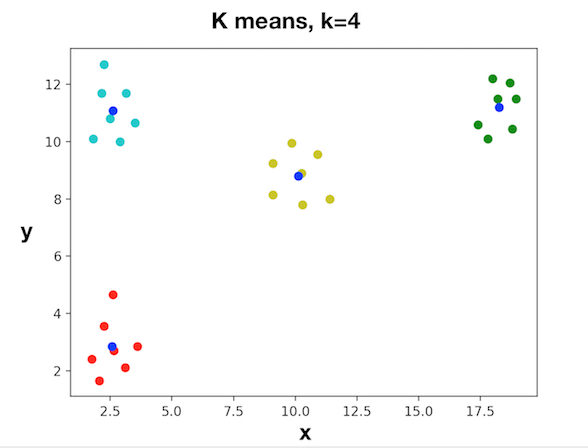
\includegraphics[width=5in]{plots/km_plot1.jpeg}\\

  Figure 2.4.2:\\
  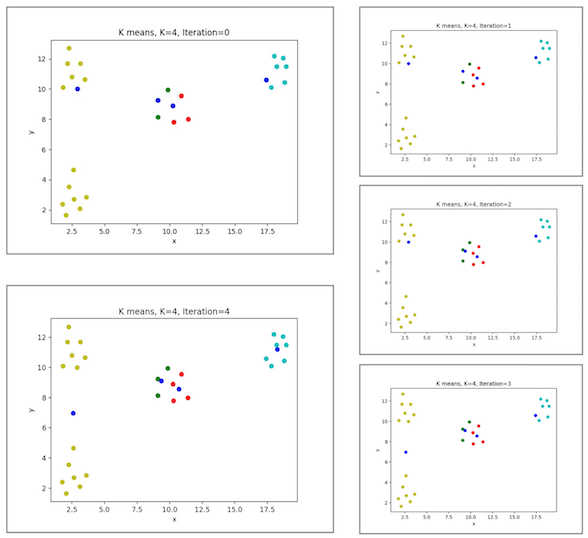
\includegraphics[width=5in]{plots/km_plot2.jpeg}\\

  Figure 2.4.3:\\
  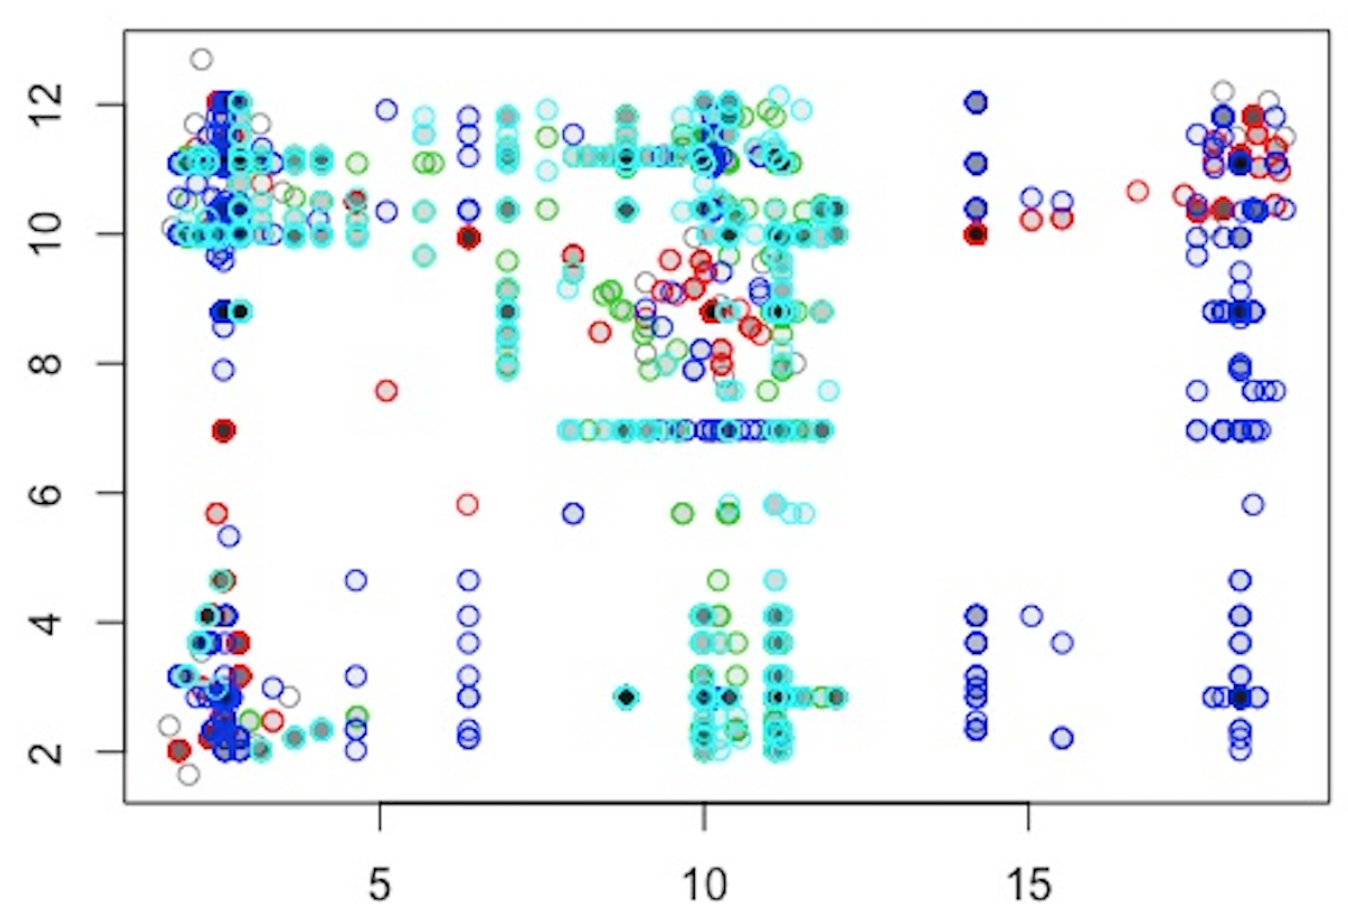
\includegraphics[width=5in]{plots/km_plot3.jpeg}\\

  Figure 2.4.4:\\
  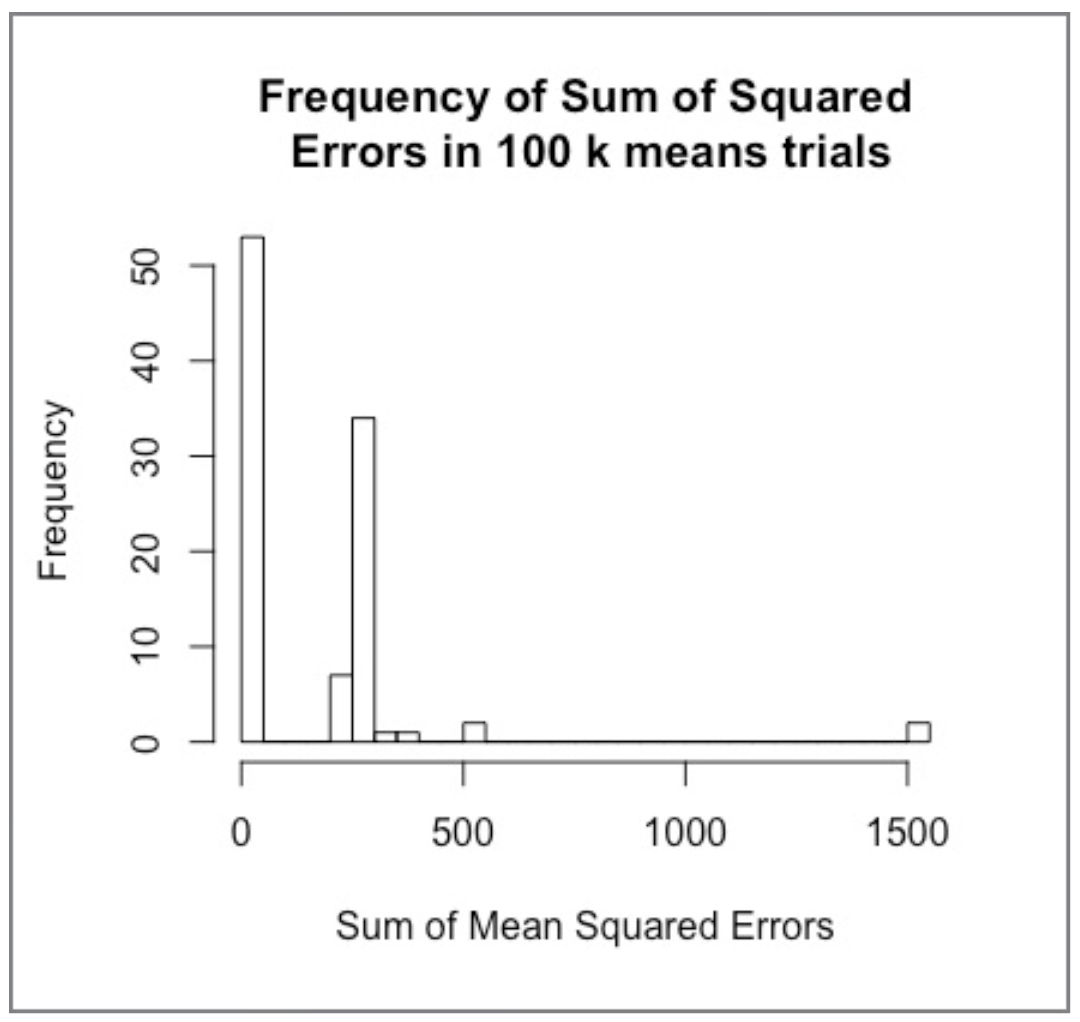
\includegraphics[width=5in]{plots/km_plot4.jpeg}\\

  Figure 2.4.5:\\
  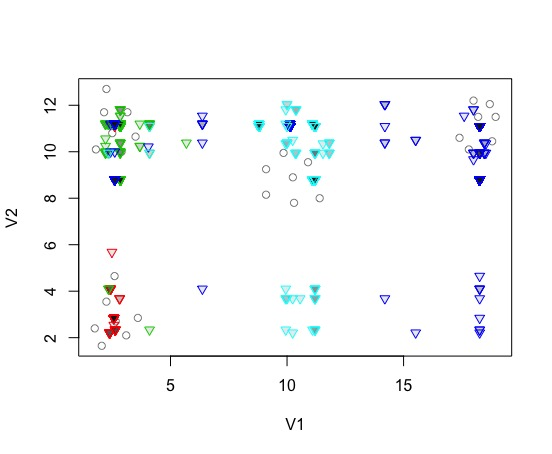
\includegraphics[width=5in]{plots/km_plot5.jpeg}\\

  Figure 2.4.6:\\
  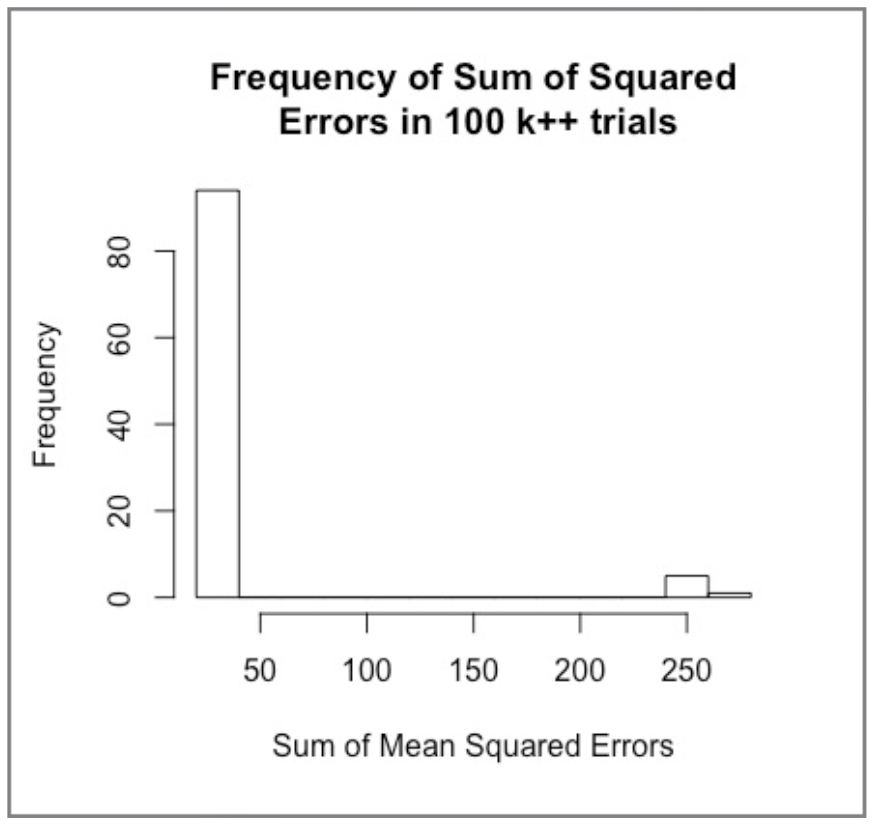
\includegraphics[width=5in]{plots/km_plot6.jpeg}\\

  Figure 2.6.1:\\
  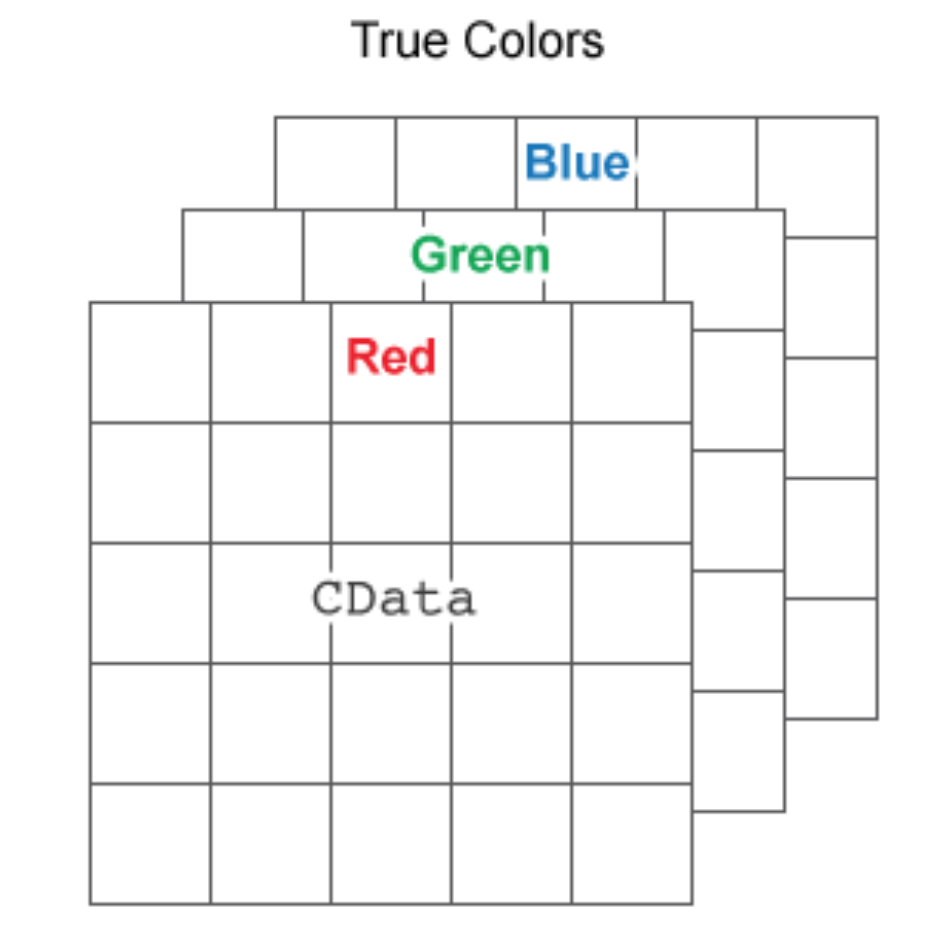
\includegraphics[width=5in]{plots/km_plot7.png}\\

  Figure 2.7.1:\\
  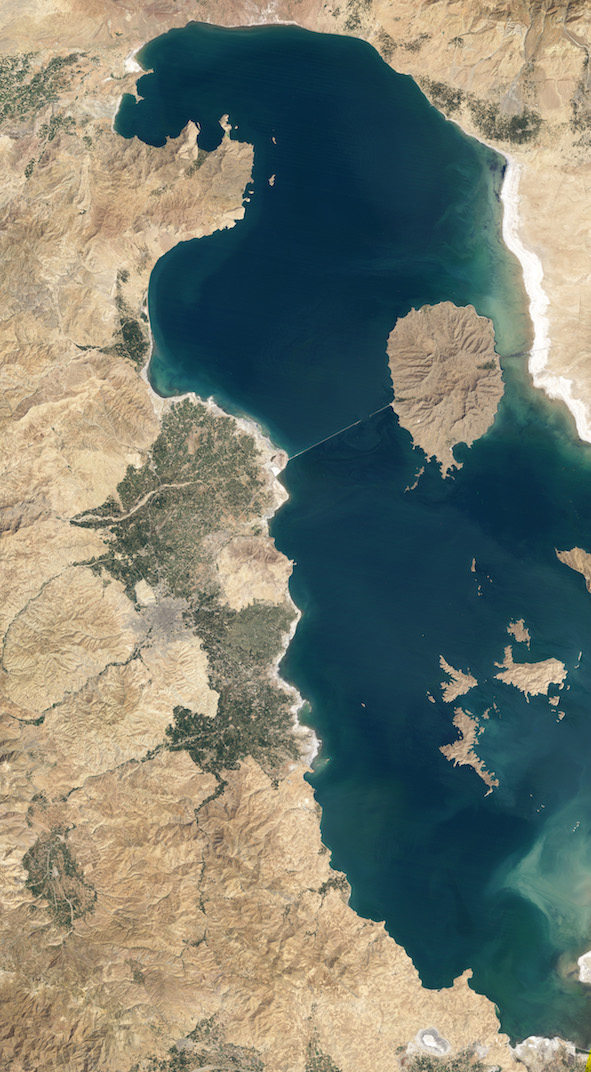
\includegraphics[width=5in]{plots/km_plot8.jpg}\\

  Figure 2.7.2:\\
  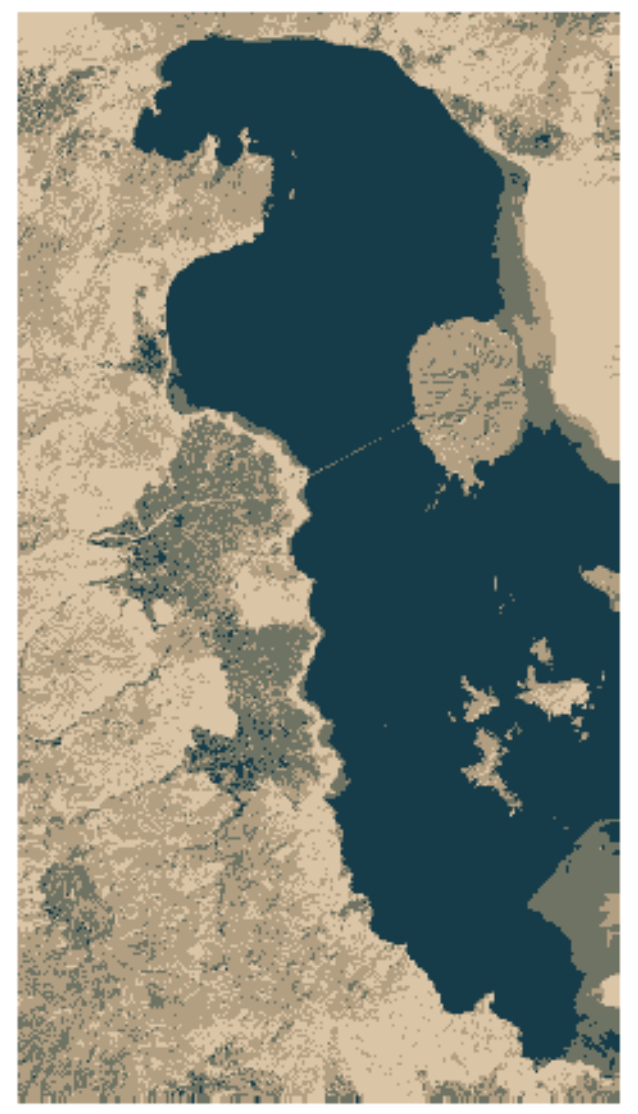
\includegraphics[width=5in]{plots/km_plot9.png}\\

  Figure 2.7.3:\\
  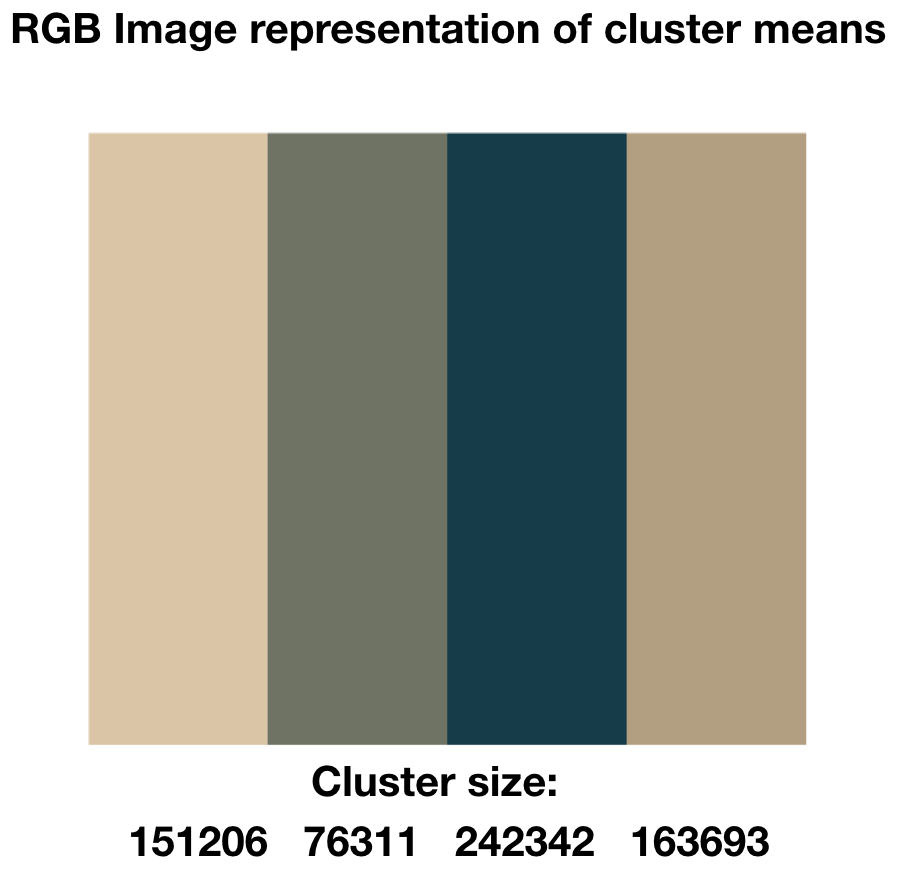
\includegraphics[width=5in]{plots/km_plot10.png}\\

  Figure 3.3.1:\\
  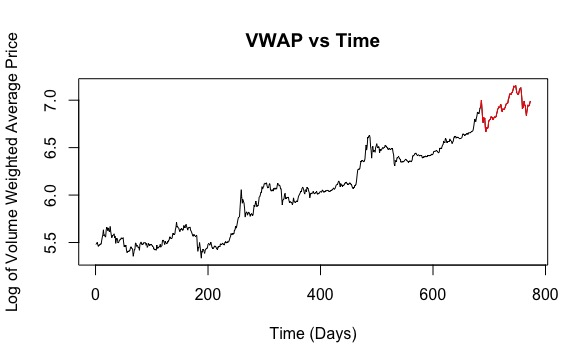
\includegraphics[width=5in]{plots/ts_plot1.jpeg}\\

  Table 3.3.1:\\
  \begin{tabular}{r|l}
    \hline
    Shape & Indicated Model \\ \hline
    Exponential, decaying to zero & AR model. Use PACF plot to help identify the order \\ \hline
    Alternating positive and negative, decaying to zero & AR model. Use the PACF plot to help identify the order \\ \hline
    One or more spikes, rest are essentially zero & MA model, order identified by where plot becomes zero \\ \hline
    Decay, starting after a few lags & Mixed autoregressive and moving average model \\ \hline
    All zero or close to zero & Data are essentially random \\ \hline
    High values at fixed intervals & Include seasonal autoregressive term \\ \hline
    No decay to zero & Series is not stationary (not differenced) \\ \hline
  \end{tabular}\\

  Figure 3.3.2:\\
  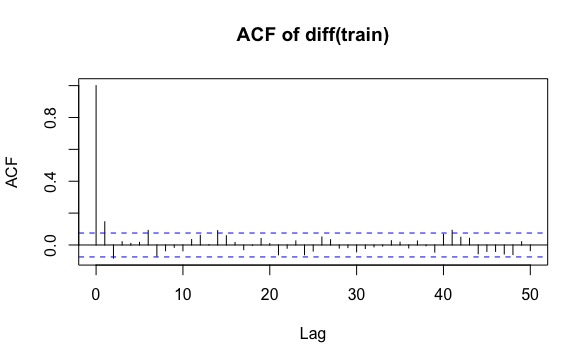
\includegraphics[width=5in]{plots/ts_plot2.jpeg}\\

  Figure 3.3.3:\\
  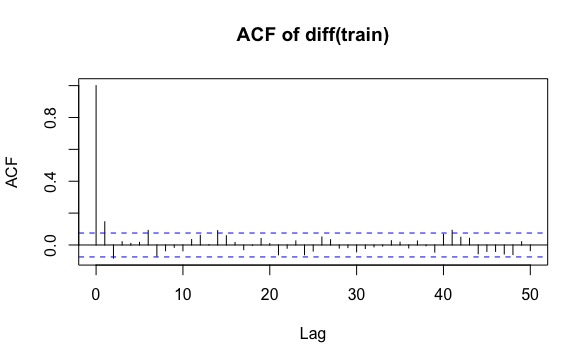
\includegraphics[width=5in]{plots/ts_plot3.jpeg}\\

  Figure 3.4.1:\\
  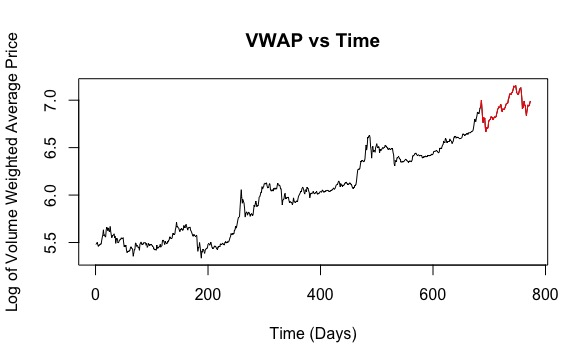
\includegraphics[width=5in]{plots/ts_plot4.jpeg}\\

  Figure 3.4.2:\\
  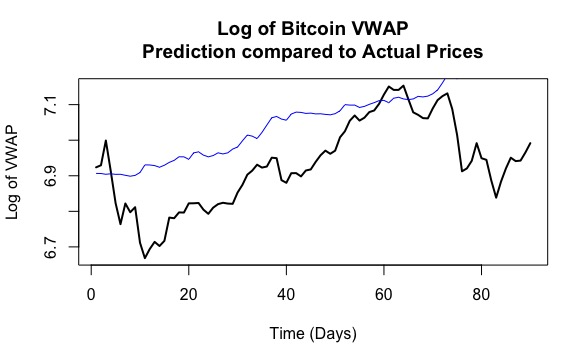
\includegraphics[width=5in]{plots/ts_plot5.jpeg}\\

  Figure 3.4.3:\\
  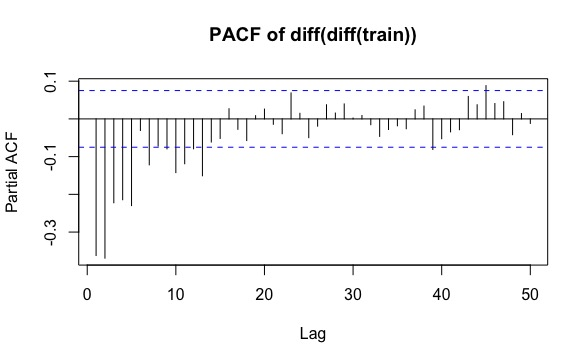
\includegraphics[width=5in]{plots/ts_plot6.jpeg}\\

  Figure 3.4.4:\\
  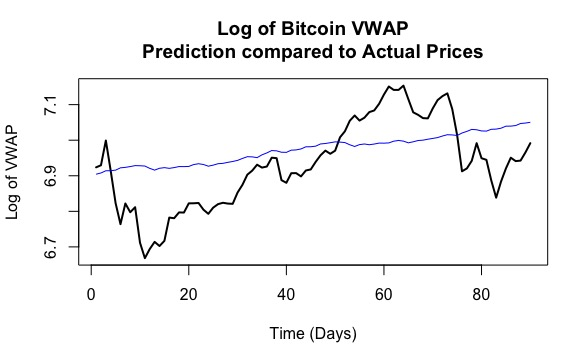
\includegraphics[width=5in]{plots/ts_plot7.jpeg}\\

  Figure 3.4.5:\\
  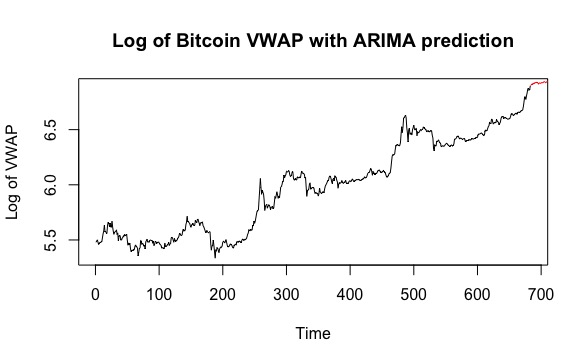
\includegraphics[width=5in]{plots/ts_plot8.jpeg}\\

  Figure 3.4.6:\\
  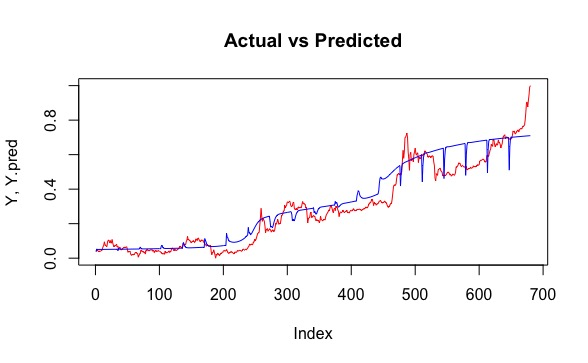
\includegraphics[width=5in]{plots/ts_plot9.jpeg}\\
  \end{center}

\pagebreak

\section {Appendix}
% ------
% R Code
% ------
\subsection{Bitcoin - Time Series Linear Regression}
\begin{minted}{r}
require(jsonlite)
require(plotly)

##############################################
# get.polo.url()
#
#   Creates a poloniex api call url
#   Either for training (train=T) or testing (train=F)
#   Testing end is 90 days past training end
#
# @param start, default=1
#   The start of your training dataset
# @param end, default=1
#   The end of your training dataset
# @param pair, default="USDT_BTC"
#   Token pairs, taken from the market list on https://poloniex.com/
# @param period, default=86400
#   Period of dataset in seconds, default=1 day
# @param train, default=TRUE
#   Whether you want the training or testing url
# @returns string
#   API URL for accessing poloniex data
##############################################
get.polo.url <- function(start=1, end=1, pair="USDT_BTC", period=86400, train=TRUE) {
  # Returns OHLC + Volume
  POLO_URL <- "https://poloniex.com/public?command=returnChartData&currencyPair=%s&start=%d&end=%d&period=%i"
  # Returns tick by tick trades (max 50000)
  # POLO_URL2 <- "https://poloniex.com/public?command=returnTradeHistory&currencyPair=%s&start=%d&end=%d"

  START <- as.numeric(as.POSIXct(sprintf("2013-%d-01", start)), tz="GMT")
  END <- as.numeric(as.POSIXct(sprintf("2017-%d-01", end)), tz="GMT")
  PRED_START <- as.numeric(as.POSIXct(sprintf("2017-%d-01", end)), tz="GMT")
  PRED_END <- as.numeric(as.POSIXct(sprintf("2017-%d-01", end)), tz="GMT")+7776000
  # PERIOD_VALUES <- c(300, 7200, 86400)
  # 5min, 2hours, 24hours
  PREDICTION_LENGTH <- 90*86400/PERIOD # days
  if(train) {
    return(sprintf(POLO_URL, pair, START, END, period))
  }
  else {
    return(sprintf(POLO_URL, pair, PRED_START, PRED_END, period))
  }
}

# -------------------------------
# Data Creation and Visualization
# -------------------------------
df <- fromJSON(get.polo.url(start=1, end=1))
pred_df <- fromJSON(get.polo.url(start=1,end=1,train=F))
train <- ts(df[8])
test <- ts(pred_df[8])

plot(log(c(train, test)), type="l", xlab="Time (Days)", ylab="Log of Volume Weighted Average Price", main="VWAP vs Time")
lines(x=seq(length(train)+1, length(train)+length(test)), y=log(test), col="red")

# -----------
# Differences
# -----------
plot(diff(train), ylab="Lagged Difference of VWAP", xlab="Time (Days)", main="diff(VWAP) vs Time")
abline(h=0)

# --------------
# ACFs and PACFs
# --------------
acf(diff(train), lag.max=50, main="ACF of diff(train)")
pacf(diff(train), lag.max=50, main="PACF of diff(train)")

# --------------------
# Model and Prediction
# --------------------
ARIMA <- arima(train, order=c(1,1,0), seasonal=list(order=c(1,1,0), period=41))
ARIMA.pred <- predict(ARIMA, n.ahead=PREDICTION_LENGTH)
error <- abs((c(test)-ARIMA.pred$pred))
error <- ((error/max(error))*(min(log(test))/max(log(test))))+min(log(test))
plot(log(test), lwd=2, xlab="Time (Days)", ylab="Log of VWAP", main="Log of Bitcoin VWAP\nPrediction compared to Actual Prices")
lines(x=seq(along=test), log(ARIMA.pred$pred), col="blue", lwd=1)
plot(log(ts(df2[8])), type='l', main="Log of Bitcoin VWAP with ARIMA prediction", ylab="Log of VWAP")
lines(x=seq(length(series)+1, length(series)+length(ARIMA.pred$pred)), y=log(ARIMA.pred$pred), col="red")

# long
#errors <- array(dim=c(4,30))
#for(i in 1:4) {
#  df <- fromJSON(get.polo.url(start=i,end=i))
#  pred_df <- fromJSON(get.polo.url(start=i,end=i,train=F))
#  train <- ts(df[8])
#  test <- ts(pred_df[8])
#  for(j in 9:38) {
#    ARIMA <- arima(train, order=c(1,1,0), seasonal=list(order=c(1,1,1), period=j))
#    ARIMA.pred <- predict(ARIMA, n.ahead=PREDICTION_LENGTH)
#    error <- sum(abs(c(test)-ARIMA.pred$pred))
#    errors[i,(j-21)] <- error
#  }
#}

# install.packages('rnn')
#library(rnn)
#TRAIN_TIME = df[1]
#TRAIN_VOLUME = df[6]
#TRAIN_PRICE = df[4]
#TEST_TIME = pred_df[1]
#TEST_VOLUME = pred_df[6]
#TEST_PRICE = pred_df[4]
\end {minted}

% ------------
% Python Codes
% ------------
\subsection{\textit{k} and \textit{k}++ means clustering}
\begin{minted}{python}
import numpy as np
import scipy
import matplotlib.pyplot as plt


class Kmeans(object):
    def __init__(self, data_as_txt, k, seed=None):
        self.k = k
        self.data_as_txt = data_as_txt
        self.seed = seed

    def load_dataset(self, name):
        return np.loadtxt(name)

    def euclidian(slef, a, b):
        return np.linalg.norm(a-b)  # magnitude between two points

    def plot(self, dataset, history_centroids, belongs_to):
        colors = ['r', 'g', 'y', 'c']

        fig, ax = plt.subplots()


        for index in range(dataset.shape[0]):
            instances_close = [i for i in range(len(belongs_to)) if belongs_to[i] == index]
            for instance_index in instances_close:
                ax.plot(dataset[instance_index][0], dataset[instance_index][1], (colors[index] + 'o'))

        history_points = []
        for index, centroids in enumerate(history_centroids):
            for inner, item in enumerate(centroids):
                if index == 0:
                    history_points.append(ax.plot(item[0], item[1], 'bo')[0])
                else:
                    history_points[inner].set_data(item[0], item[1])
                    plt.pause(0.8)


    ''' num_instances: number of rows in data (i.e how many points)
        dataset: the data
        return: list of k randomly selected data points in a list: [[x1 y1] [x2 y2] ... [xk yk]]
    '''
    def initialization(self, dataset):

        if self.seed is not None:
            np.random.seed(self.seed)

        num_instances, num_features = dataset.shape  # 45, 2
        return dataset[np.random.choice(num_instances - 1, self.k, replace=False)]
        #return dataset[np.random.randint(0, num_instances - 1, size = self.k)]

    def kmeans(self, k, epsilon=0, distance='euclidian'):
        history_centroids = []
        if distance == 'euclidian':
            dist_method = self.euclidian
        dataset = self.load_dataset(self.data_as_txt)
        # dataset = dataset[:, 0:dataset.shape[1] - 1]
        num_instances, num_features = dataset.shape  # 45, 2


        #prototypes = dataset[np.random.randint(0, num_instances - 1, size=k)]
        prototypes = self.initialization(dataset)
        history_centroids.append(prototypes)
        prototypes_old = np.zeros(prototypes.shape)
        belongs_to = np.zeros((num_instances, 1))
        norm = dist_method(prototypes, prototypes_old)
        iteration = 0

        while norm > epsilon:
            iteration += 1
            norm = dist_method(prototypes, prototypes_old)
            prototypes_old = prototypes
            for index_instance, instance in enumerate(dataset):
                dist_vec = np.zeros((k, 1))
                for index_prototype, prototype in enumerate(prototypes):
                    dist_vec[index_prototype] = dist_method(prototype,
                                                            instance)

                belongs_to[index_instance, 0] = np.argmin(dist_vec)

            tmp_prototypes = np.zeros((k, num_features))

            for index in range(len(prototypes)):
                instances_close = [i for i in range(len(belongs_to)) if belongs_to[i] == index]
                prototype = np.mean(dataset[instances_close], axis=0)
                # prototype = dataset[np.random.randint(0, num_instances, size=1)[0]]

                tmp_prototypes[index, :] = prototype

            prototypes = tmp_prototypes

            history_centroids.append(tmp_prototypes)

        #self.plot(dataset, history_centroids, belongs_to)

        return prototypes, history_centroids, belongs_to

    def execute(self, graph=True):
        dataset = self.load_dataset(self.data_as_txt)
        centroids, history_centroids, belongs_to = self.kmeans(self.k)
        if(graph):
            self.plot(dataset, history_centroids, belongs_to)

        return centroids


class Kpp(Kmeans):

    def initialization(self, dataset):
        X = dataset
        print(X)

        C = [X[0]]
        print(C)
        for k in range(1, self.k):
            #  find shortest distantce squared to center
            D2 = scipy.array([min([scipy.inner(c-x, c-x) for c in C]) for x in X])
            probs = D2/D2.sum()
            cumprobs = probs.cumsum()
            print(cumprobs)
            r = scipy.rand()
            for j, p in enumerate(cumprobs):
                if r < p:
                    i = j
                    break
            C.append(X[i])
        return np.array(C)

if __name__ == "__main__":
    kpp_means = Kpp("pts2.txt", 4)
    #centroids = kpp_means.execute(graph=True)

    kmeans = Kmeans("pts2.txt", 4)
    #centroids = kmeans.execute(graph=True)

    all_kmeans_centroids = []
    all_kpp_means_centroids = []

    for _ in range(1, 1000):
        kmeans_centroids = kmeans.execute(graph=False)
        all_kmeans_centroids.append(kmeans_centroids)

    for _ in range(1, 1000):
        kpp_centroids = kpp_means.execute(graph=False)
        all_kpp_means_centroids.append(kpp_centroids)

    with open("KmeansCentroids.txt", mode='w') as File:
        for i in all_kmeans_centroids:
            for j in i:
                File.write("{} {} ".format(j[0], j[1]))
            File.write("\n")

    with open("KppCentroids.txt", mode='w') as File:
        for i in all_kpp_means_centroids:
            for j in i:
                File.write("{} {} ".format(j[0], j[1]))
            File.write("\n")
\end{minted}

% ------
% R code
% ------
\subsection {Centroid Plots and Distribution of SSE}
\begin{minted}{r}
# --------------
# Plot centroids
# --------------
points <- read.table("pts2.txt")
kmeansCentroids <- read.csv("KmeansCentroids.txt", sep=" ", header=FALSE, na.strings="nan")[1:8]
kppCentroids <- read.csv("KppCentroids.txt", sep=" ", header=FALSE, na.strings="nan")[1:8]

plot(points, col=rgb(0,0,0,0.5))
for(i in 1:4) {
  points(x=kmeansCentroids[,1*i], y=kmeansCentroids[,2*i], pch=21, col=i+1, bg=rgb(0.1,0.1,0.1,0.1))
}
plot(points, col=rgb(0,0,0,0.5))
for(i in 1:4) {
  points(x=kppCentroids[,1*i], y=kppCentroids[,2*i], pch=25, col=i+1, bg=rgb(0.1,0.1,0.1,0.1))

# ------------------------
# Show distribution of SSE
# ------------------------
x <- read.csv("kmeans_sse.csv", sep=" ", header=FALSE)
x <- unlist(x, use.names=FALSE)
hist(x, main="Frequency of Sum of Mean Squared\n Errors in 100 k means trials", xlab="Sum of Mean Squared Errors", breaks=100)
mu <- mean(x)
variance <- var(x)
print(mu)
print(variance)
print(IQR(x))

x <- read.csv("kpp_sse.csv", sep=" ", header=FALSE)
x <- unlist(x, use.names=FALSE)
hist(x, main="Frequency of Sum of Mean Squared\n Errors in 100 k++ trials", xlab="Sum of Mean Squared Errors", breaks=100)
mu <- mean(x)
variance <- var(x)
print(mu)
print(variance)
print(IQR(x))
\end{minted}

% Link to repo
GitHub repository for code: \url{https://github.com/immackay/4990-Final-Project}
% Bibliography
\pagebreak
\bibliographystyle{plain}
\bibliography{sources}

\end{document}
